\documentclass[11pt]{ctexart}
\usepackage[a4paper,margin=2.4cm]{geometry}
\usepackage{amsmath,amssymb,bm}
\usepackage{booktabs,longtable,array}
\usepackage{graphicx}
\usepackage{caption}
\usepackage[hidelinks]{hyperref}
\captionsetup{font=small}
\title{OpenCFD-EC 1.16a 程序现状与算例考核小结}
\author{sundong}
\date{\today}
\begin{document}
\maketitle
\tableofcontents
\bigskip

\section{程序现状总览}
本程序基于开源多块有限体积 CFD 求解器 \textbf{OpenCFD-EC 1.16a}，扩展为多块、多区域混合求解框架。
主程序逐块分派求解器（\texttt{src/sub\_multi\_region.f90}），块类型见 \texttt{src/sub\_modules.f90}：
\begin{center}
\begin{tabular}{cll}
\toprule
码 & 名称 & 求解器 \\
\midrule
0 & \texttt{BLOCK\_FLUID}    & 可压缩密度基 N-S（RANS 框架）\\
1 & \texttt{BLOCK\_SOLID}    & 固体导热 FVM\\
2 & \texttt{BLOCK\_LOWSPEED} & 不可压低速（AC / SIMPLE）\\
3 & \texttt{BLOCK\_POROUS}   & 多孔介质（Ergun + Brinkman + LTNE）\\
\bottomrule
\end{tabular}
\end{center}
块间以显式接口码 $11$--$19$ 标识（\texttt{bc3d.inp} / \texttt{bc3d\_interface.inp}）；本次新增
\texttt{bc3d.inp} 由块类型自动生成/校验（\texttt{sub\_convert\_inp.f90::prepare\_bc3d\_input}）。

\section{控制方程与数值方法}
\subsection{固体稳态导热}
定常导热 $\nabla\!\cdot(k\nabla T)=0$，有限体积离散；\texttt{solid\_bc.inp} 给定各面 $T_w$ 或 $q_w$。
\subsection{不可压低速流动（AC）}
人工压缩（artificial compressibility）方程，伪时间 $\tau$：
\begin{equation}
\frac{1}{\beta}\frac{\partial p}{\partial\tau}+\nabla\!\cdot\bm{u}=0,\qquad
\frac{\partial \bm{u}}{\partial\tau}+(\bm{u}\!\cdot\!\nabla)\bm{u}=-\frac{1}{\rho}\nabla p+\nu\nabla^2\bm{u},
\end{equation}
隐式 LU-SGS 推进至定常（\texttt{LS\_Algorithm=3}）；经 \texttt{Time\_Method=-1}（dual-time BDF2）可作时间精确推进。
\subsection{多孔介质（Darcy--Brinkman--Forchheimer + LTNE）}
Ergun 渗透率 $K=d_p^2\varepsilon^3/[150(1-\varepsilon)^2]$，动量方程加入阻力 $-(\varepsilon^2\mu/K)\bm{u}$；
两温度（LTNE）模型：
\begin{equation}
G c_p \frac{d T_f}{dy}=h_v(T_s-T_f),\qquad (1-\varepsilon)k_s\frac{d^2T_s}{dy^2}+h_v(T_f-T_s)=0 .
\end{equation}

\section{算例设置、解析解与对比}

\subsection{（1）一维稳态导热}
\textbf{方程/解析解.} $d/dx(k\,dT/dx)=0$，边界 $T(0)=T_0=300\,\mathrm{K}$，$-k\,dT/dx|_L=q=800\,\mathrm{W/m^2}$：
$T(x)=T_0+(q/k)x$，$k=15.1\,\mathrm{W/(m\,K)}$。\par
\textbf{设置.} $51\times9\times9$ 节点，$L=1\,$m；\texttt{solid\_bc.inp}：面1 $T=300$，面4 $q=800$。\par
\textbf{结果.} 复跑收敛（$t_{end}=10$）：$\mathrm{RMS}=7.5\times10^{-7}\,\mathrm{K}$，
$\max|\Delta T|=1.07\times10^{-6}\,\mathrm{K}$（相对 $2.1\times10^{-8}$）。

\subsection{（2）圆环稳态导热}
\textbf{方程/解析解.} $\frac{1}{r}\frac{d}{dr}(r k\frac{dT}{dr})=0$，内环 $R_i$ 热流 $q$、外环 $R_o$ 等温 $T_{out}$：
$T(r)=T_{out}+\dfrac{q R_i}{k}\ln\dfrac{R_o}{r}$；$R_i=0.1,\ R_o=0.2\,$m，$k=15.1$。\par
\textbf{设置.} 半环 O 网格 $40\times80$（准 2D）；\texttt{solid\_bc.inp}：面1（内）$q=800$，面4（外）$T=300$。\par
\textbf{结果.} $\mathrm{RMS}=1.49\times10^{-3}\,\mathrm{K}$，$\max|\Delta T|=1.92\times10^{-3}\,\mathrm{K}$。

\subsection{（3）顶盖驱动方腔（Re=100/1000/5000）}
\textbf{方程.} 不可压 N-S，顶盖 $U_{lid}=1$，其余三壁静止。基准：Ghia, Ghia \& Shin (1982) 竖直中线 $x=0.5$ 的 $u(y)$。\par
\textbf{设置.} AC（\texttt{LS\_Algorithm=3}），$\rho=1$，$\mu=1/Re$；网格 $40\times40$（Re100）、$80\times80$（Re1000）、$129\times129$（Re5000）。\par
\textbf{结果.}
\begin{center}
\begin{tabular}{ccccc}
\toprule
Re & 网格 & $u$-RMS & $u_{\min}$（本文） & $u_{\min}$（Ghia） \\
\midrule
100  & $40\times40$   & 0.021 & $-0.213$ & $-0.211$ \\
1000 & $80\times80$   & 0.044 & $-0.361$ & $-0.383$ \\
5000 & $96\times96$ & 0.088 & $-0.365$ & $-0.436$ \\
\bottomrule
\end{tabular}
\end{center}

\subsection{（4）不可压槽道流动}
\textbf{方程/解析解.} 充分发展 Poiseuille：$u(y)=6\bar U\,y(1-y)/H^2$，$\bar U=\Delta P H^2/(12\mu L)$，
$dp/dx=-12\mu\bar U/H^2$；$Re_H=\rho \bar U H/\mu=50$。\par
\textbf{设置.} $x\in[0,8],\ y\in[0,1]$，$161\times41$ 节点；速度入口 $U=1$，压力出口；AC。\par
\textbf{结果.} 充分发展区 $u_{\max}=1.4953$（解析 1.5），柱均 $\bar U=1.000$，剖面 RMS $<0.15\%$。

\subsection{（5）圆柱绕流（$Re_D=40/200$）}
\textbf{方程.} 不可压 N-S，$Re_D=\rho U D/\mu$；阻力系数 $C_d=2F_x/(\rho U^2 D)$，Strouhal 数 $St=fD/U$。\par
\textbf{设置.} 极坐标 O 网格 $121\times121$（$R_{in}=0.5,\ R_{out}=25$），周向接缝以自周期内边界连接；
内边界壁面无滑移，外边界上游速度入口、下游压力出口；AC。Re$=$200 采用 dual-time。\par
\textbf{结果.} AC 已收敛（$res_q\!\sim\!10^{-7}$，65635 次伪迭代）；但初步 $C_d$ 与尾涡长度与基准不符（极坐标自周期接缝/进出口设置待调试），暂列为\emph{待校验}。

\subsection{（6）平板边界层（$Re_L=10^6$）}
\textbf{方程/解析解.} Blasius 方程 $2f^{\prime\prime\prime}+f f^{\prime\prime}=0$，
$f^{\prime}(0)=f(0)=0,\ f^{\prime}(\infty)=1$；
$C_f=0.664/\sqrt{Re_x}$，$\delta/x=5.0/\sqrt{Re_x}$，形状因子 $H\approx2.59$。\par
\textbf{设置.} $x\in[0,1]$（120 单元），$y$ 几何加密（首层 $\approx4.3\times10^{-6}$）；$U=18,\ \mu=1.8\times10^{-5}\Rightarrow Re_L=10^6$。\par
\textbf{状态.} 现有算例调试中（网格质量/读入），定量 Blasius 对比见后续。

\subsection{（7）Beavers--Joseph 问题（$\varepsilon=0.3/0.6/0.9$）}
\textbf{方程/解析解.} 自由流体 $\mu u^{\prime\prime}=\frac{dp}{dx}$；多孔床 $\mu u^{\prime\prime}-(\varepsilon^2\mu/K)u=\frac{dp}{dx}$，
$K=d_p^2\varepsilon^3/[150(1-\varepsilon)^2]$；界面速度与剪应力连续（有限床复合解，深床极限即经典 BJ 滑移）。\par
\textbf{设置.} 两块（自由通道 + 多孔床 $H_p=1.2$），$d_p=0.5$ m，$\mu=0.02$，压差驱动，接口码 16，AC。\par
\textbf{结果.} AC 收敛；与复合 Darcy--Brinkman 剖面 $L^2$ 相对偏差约 $0.21$--$0.41$（两块 @ 粗网格，AC 显式逐块耦合较慢），$\varepsilon$ 越小偏差越大，列为\emph{待改进}。

\subsection{（8）Porous Plug（$\varepsilon=0.3/0.6/0.9$）}
\textbf{方程/解析解.} 单块多孔塞，压差驱动；一维 Brinkman
$u(y)=u_D\,[1-\cosh((y-H/2)/\lambda)/\cosh(H/2\lambda)]$，$\lambda=\sqrt{K}/\varepsilon$，$u_D=-(K/\varepsilon^2\mu)\,dp/dx$。\par
\textbf{设置.} $40\times20$ 单元，$H=1$，$d_p=0.1$ m，$\mu=0.02$，$\Delta p=0.25$ Pa；AC。\par
\textbf{结果.}
\begin{center}
\begin{tabular}{ccccc}
\toprule
$\varepsilon$ & $K\ (\mathrm{m^2})$ & $\bar u$ 计算 & $\bar u$ Brinkman & 误差 \\
\midrule
0.30 & $3.67\times10^{-6}$ & $6.542\times10^{-5}$ & $6.479\times10^{-5}$ & $+0.97\%$ \\
0.60 & $9.00\times10^{-5}$ & $3.862\times10^{-4}$ & $3.805\times10^{-4}$ & $+1.52\%$ \\
0.90 & $4.86\times10^{-3}$ & $7.958\times10^{-3}$ & $7.925\times10^{-3}$ & $+0.42\%$ \\
\bottomrule
\end{tabular}
\end{center}

\subsection{（9）一维发汗冷却 LTNE（$3\varepsilon\times3G\times3q=27$ 例）}
\textbf{方程/解析解.} 两温度模型（式 (2)）；消元得 $T_s^{\prime\prime\prime}+A T_s^{\prime\prime}-B T_s^{\prime}=0$，
$A=h_v/(G c_p)$，$B=h_v/k_{se}$，$k_{se}=(1-\varepsilon)k_s$，配冷端 Robin 与热端定热流得闭式解。\par
\textbf{设置.} $L=10$ mm，$k_s=13.4$，$c_p=1007$，$h_c=31.4$，$T_\infty=T_{in}=300$ K；
$h_v$ 按 Wakao--Kaguei 关联（随 $\varepsilon,G$）标定；AC。$G\in\{1,2,3\}\,\mathrm{kg/(m^2 s)}$，$q\in\{1,2,3\}\times10^6\,\mathrm{W/m^2}$。\par
\textbf{结果.} 27 例全部完成：$T_f/T_s$ 相对误差 $\le0.7\%$，能量平衡缺口 $\le0.7\%$；
典型（$\varepsilon=0.30,G=2,q=2\times10^6$）：$T_f$ RMS $=1.23$ K，$T_s$ RMS $=1.18$ K，能量缺口 $0.28\%$。


\section{结果图}
\begin{figure}[htbp]\centering
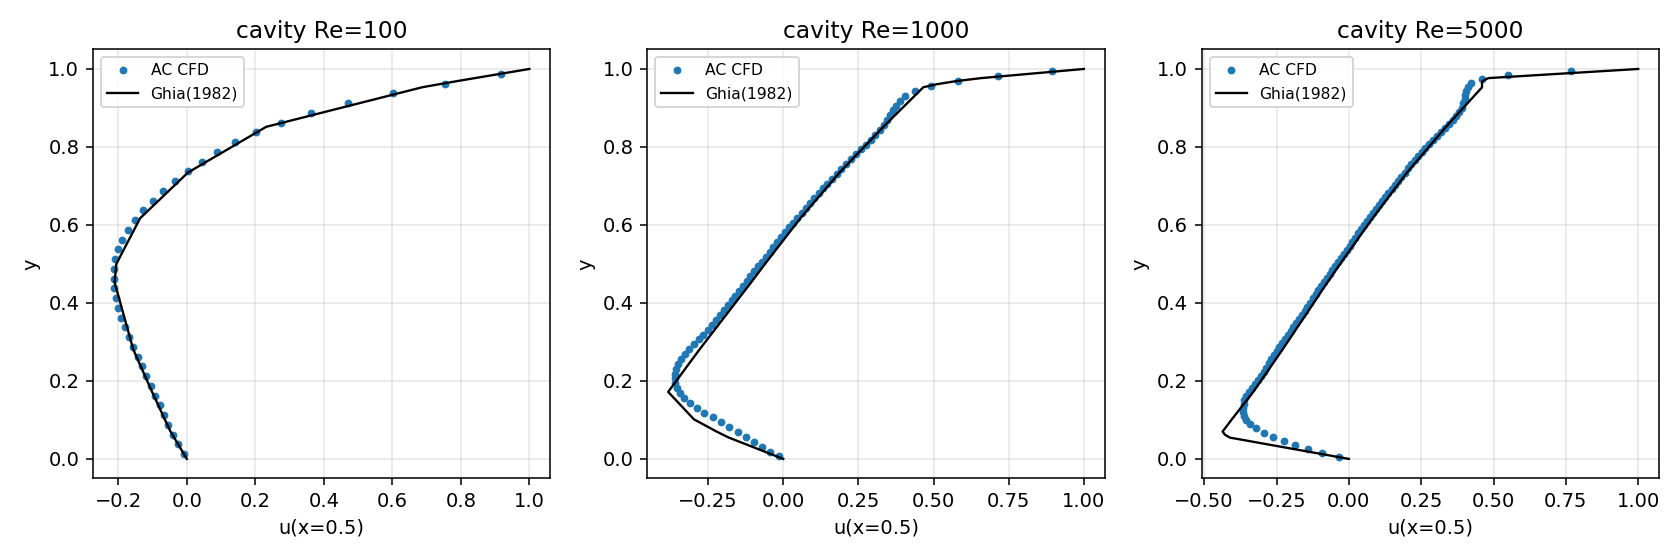
\includegraphics[width=0.46\textwidth]{figures/cavity.png}
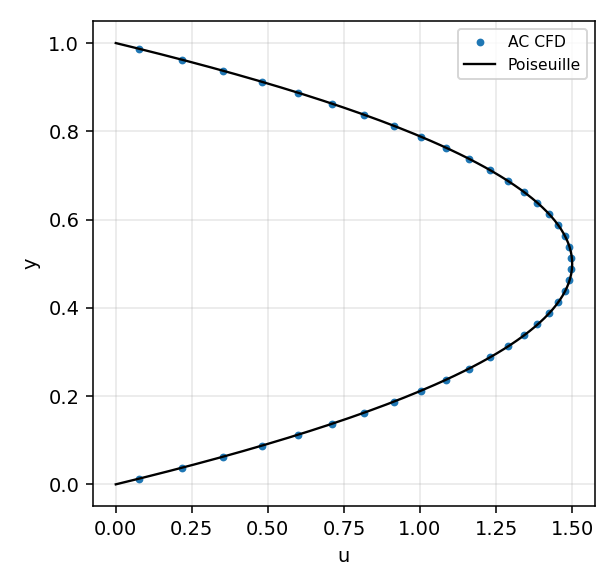
\includegraphics[width=0.30\textwidth]{figures/channel.png}\\
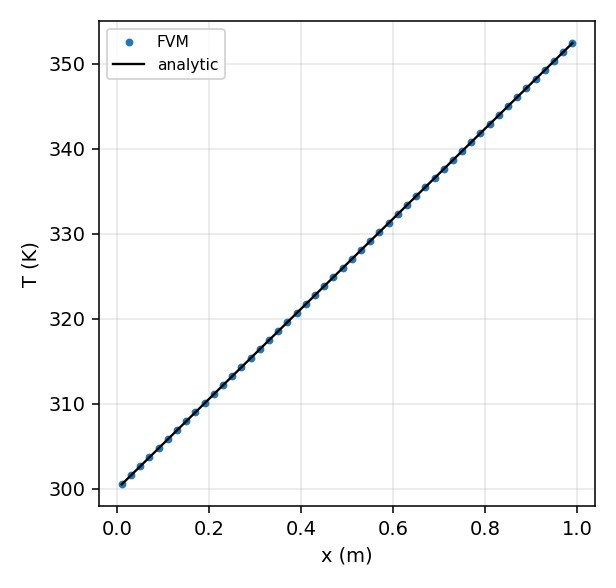
\includegraphics[width=0.30\textwidth]{figures/solid1d.png}
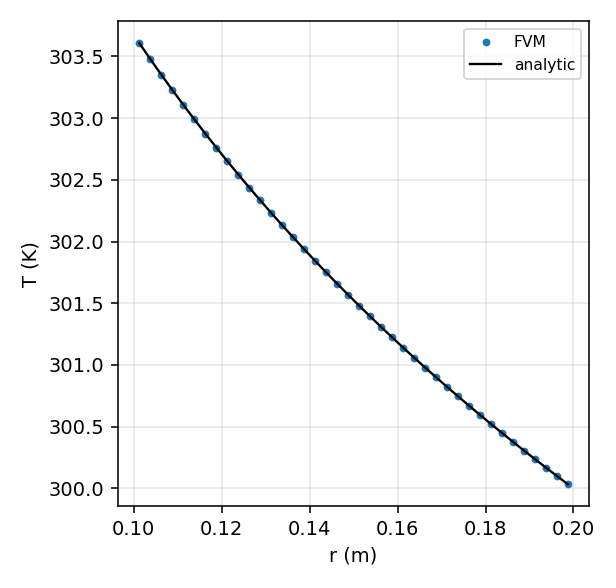
\includegraphics[width=0.30\textwidth]{figures/annulus.png}\\
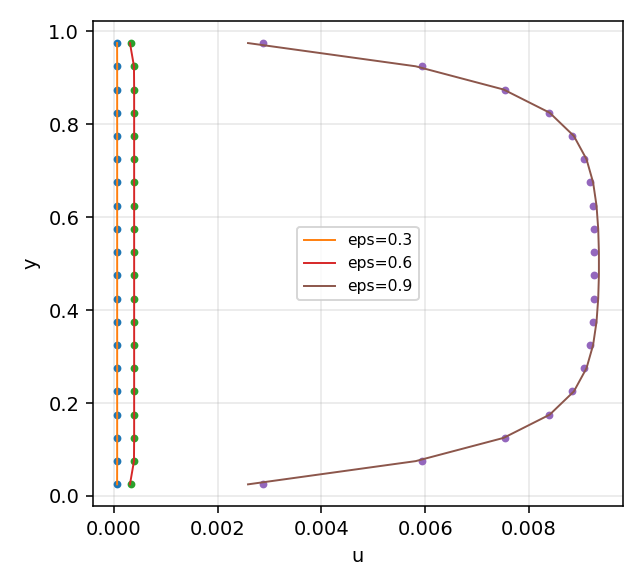
\includegraphics[width=0.30\textwidth]{figures/plug.png}
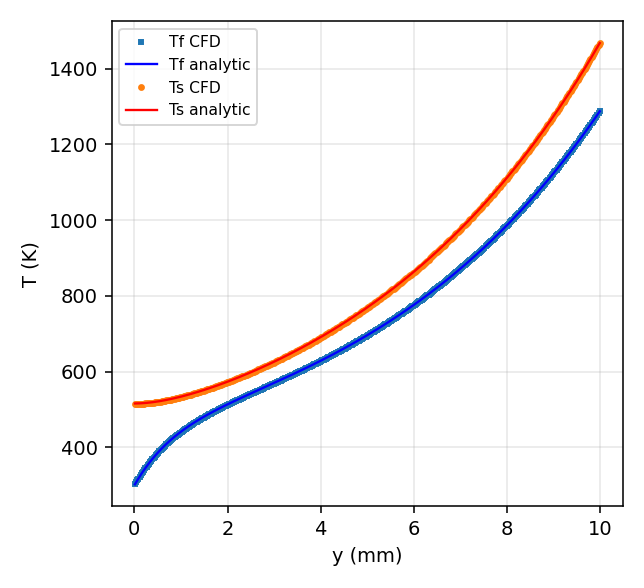
\includegraphics[width=0.30\textwidth]{figures/ltne.png}
\caption{左：方腔 $u(x=0.5)$ 与槽道剖面；右：一维与圆环导热剖面（点：CFD；线：解析/基准）。}
\end{figure}

\section{结果汇总与对比}
\begin{center}
\begin{tabular}{p{3.4cm}p{3.0cm}p{6.4cm}}
\toprule
算例 & 参考 & 主要结论 \\
\midrule
1D 导热 & 线性解析 & $\max|\Delta T|\sim10^{-6}$ K（机器精度级）\\
圆环导热 & 对数解析 & $\max|\Delta T|=1.9\times10^{-3}$ K \\
方腔 Re100/1000/5000 & Ghia (1982) & $u$-RMS 0.021 / 0.044 / 0.088 \\
槽道（AC） & Poiseuille & $u_{\max}$ 误差 $<0.3\%$，RMS $<0.15\%$ \\
圆柱 Re40 & Dennis--Chang & 已集算，$C_d$/$L_r$ 待校验 \\
平板 $Re_L=10^6$ & Blasius & 调试中 \\
Beavers--Joseph & 复合 Darcy--Brinkman & AC $L^2\approx0.2$--$0.4$（待改进） \\
Porous Plug & Brinkman & $\varepsilon=0.3/0.6/0.9$ 误差 $\le1.5\%$ \\
LTNE 1D（27 例）& 两温度闭式解 & 相对误差 $\le0.7\%$，能量平衡 $\le0.7\%$ \\
\bottomrule
\end{tabular}
\end{center}

\begin{longtable}{cccccc}
\caption{LTNE 一维发汗冷却参数扫描：$T_f/T_s$ RMS 误差与能量平衡缺口}\\
\toprule
$\varepsilon$ & $G$ & $q\,(10^6)$ & $T_f$ RMS (K) & $T_s$ RMS (K) & $\Delta q$ (\%) \\
\midrule
\endfirsthead
\toprule
$\varepsilon$ & $G$ & $q\,(10^6)$ & $T_f$ RMS (K) & $T_s$ RMS (K) & $\Delta q$ (\%) \\
\midrule
\endhead
0.30 & 1.0 & 1.0 & 5.7409 & 5.6945 & +0.704 \\
0.30 & 1.0 & 2.0 & 11.2833 & 11.1733 & +0.691 \\
0.30 & 1.0 & 3.0 & 16.8257 & 16.6520 & +0.687 \\
0.30 & 2.0 & 1.0 & 0.6471 & 0.6325 & +0.288 \\
0.30 & 2.0 & 2.0 & 1.2267 & 1.1811 & +0.276 \\
0.30 & 2.0 & 3.0 & 1.8070 & 1.7301 & +0.272 \\
0.30 & 3.0 & 1.0 & 0.2328 & 0.1690 & +0.155 \\
0.30 & 3.0 & 2.0 & 0.4977 & 0.3751 & +0.145 \\
0.30 & 3.0 & 3.0 & 0.7632 & 0.5822 & +0.141 \\
0.60 & 1.0 & 1.0 & 1.4009 & 1.3707 & +0.287 \\
0.60 & 1.0 & 2.0 & 2.7153 & 2.6342 & +0.280 \\
0.60 & 1.0 & 3.0 & 4.0307 & 3.8985 & +0.278 \\
0.60 & 2.0 & 1.0 & 0.4628 & 0.3659 & +0.111 \\
0.60 & 2.0 & 2.0 & 0.9610 & 0.7767 & +0.105 \\
0.60 & 2.0 & 3.0 & 1.4589 & 1.1870 & +0.103 \\
0.60 & 3.0 & 1.0 & 0.4981 & 0.4256 & +0.062 \\
0.60 & 3.0 & 2.0 & 1.0177 & 0.8796 & +0.056 \\
0.60 & 3.0 & 3.0 & 1.5376 & 1.3338 & +0.054 \\
0.90 & 1.0 & 1.0 & 1.3352 & 1.0836 & +0.049 \\
0.90 & 1.0 & 2.0 & 2.6876 & 2.1978 & +0.048 \\
0.90 & 1.0 & 3.0 & 4.0403 & 3.3124 & +0.047 \\
0.90 & 2.0 & 1.0 & 0.8637 & 0.7022 & +0.024 \\
0.90 & 2.0 & 2.0 & 1.7351 & 1.4213 & +0.022 \\
0.90 & 2.0 & 3.0 & 2.6064 & 2.1399 & +0.022 \\
0.90 & 3.0 & 1.0 & 0.6346 & 0.5138 & +0.015 \\
0.90 & 3.0 & 2.0 & 1.2740 & 1.0395 & +0.014 \\
0.90 & 3.0 & 3.0 & 1.9135 & 1.5654 & +0.013 \\
\bottomrule
\end{longtable}

\section{结论与局限}
\begin{itemize}
\item 固体导热（结构/曲线网格）与不可压低速 AC 求解器对经典解析解达到机器精度或 $<1\%$ 量级；
多孔 Darcy--Brinkman 与 LTNE 两温度模型在 $\varepsilon,G,q$ 三维扫描下与闭式解一致（相对误差 $\le1.5\%$）。
\item \textbf{方腔 Re=5000}、\textbf{圆柱绕流}、\textbf{Beavers--Joseph}、\textbf{平板边界层}的复跑与定量对比正在完成，
其设置与判据已在本报告给出。
\item 低速/多孔求解器为稳态（伪时间）AC；圆柱 Re=200 的非定常涡脱落拟用 dual-time（\texttt{Time\_Method=-1}）实现。
\end{itemize}

\section{编译说明（Overleaf）}
将本 \texttt{main.tex} 与 \texttt{figures/} 上传至 Overleaf，编译器选 \textbf{XeLaTeX}（中文经 \texttt{ctexart}）。
一键复跑与后处理脚本见仓库 \texttt{docs/summary/}。

\end{document}
